\chapter{Вычислительные эксперименты}
\section{Алгоритм решения}
Для построения математической модели введём замену переменных $\beta(t) = \dot{\alpha}(t)$, что позволяет записать исходное уравнение во втором порядке в виде системы дифференциальных уравнений первого порядка:

\[
\begin{cases}
	\dot{\beta} = -\omega^2 \sin \alpha, \\
	\dot{\theta} = \beta, \\
	\beta(0) = \theta_1, \quad \theta(0) = \alpha_0.
\end{cases}
\]
Или для линейной модели :
\[
\begin{cases}
	\dot{\beta} = -\omega^2 \alpha, \\
	\dot{\theta} = \beta, \\
	\beta(0) = \theta_1, \quad \theta(0) = \theta_0.
\end{cases}
\]

Аналогичным образом уравнения, включающие внешние воздействия, можно привести к этому же виду.

Для численного решения данной системы будем использовать метод Рунге-Кутты\cite{1964calculus}, что позволит получить решение с заданными параметрами. 

Метод Рунге-Кутты четвертого порядка (RK4) обладает порядком точности \( O(h^4) \), что означает, что ошибка метода уменьшается пропорционально четвертой степени размера шага \( h \). 

После вычисления построим фазовый портрет и график изменения угла во времени.

\section{Программа для ЭВМ}
В качестве языка программирования для рассчётов и визуализации был выбран Python с использованием библиотек numpy (вычисления) и matplotlib (визуализация).
С использованием этих инструментов была написана программа (Листинг \ref{lst:sample01}) для ЭВМ.
\lstinputlisting[language=Python,
caption=Код программы (\Code{pendulum.py}),label={lst:sample01}
]{./listings/main.py} 

Зададим $L = 1\text{м}$, тогда собственная частота будет равна : $\omega = \sqrt\frac{g}{L} \approx 3.13$.
\section{Результаты  экспериментов}
\subsection*{Модель без дополнительных сил}
Сравним линейную и нелинейную модель при разных углах наклона и нулевой начальной скорости. Промежуток времени $[0,25]$, шаг - 0.025:
\begin{figure}[h]  % Окружение для картинки
	\centering
	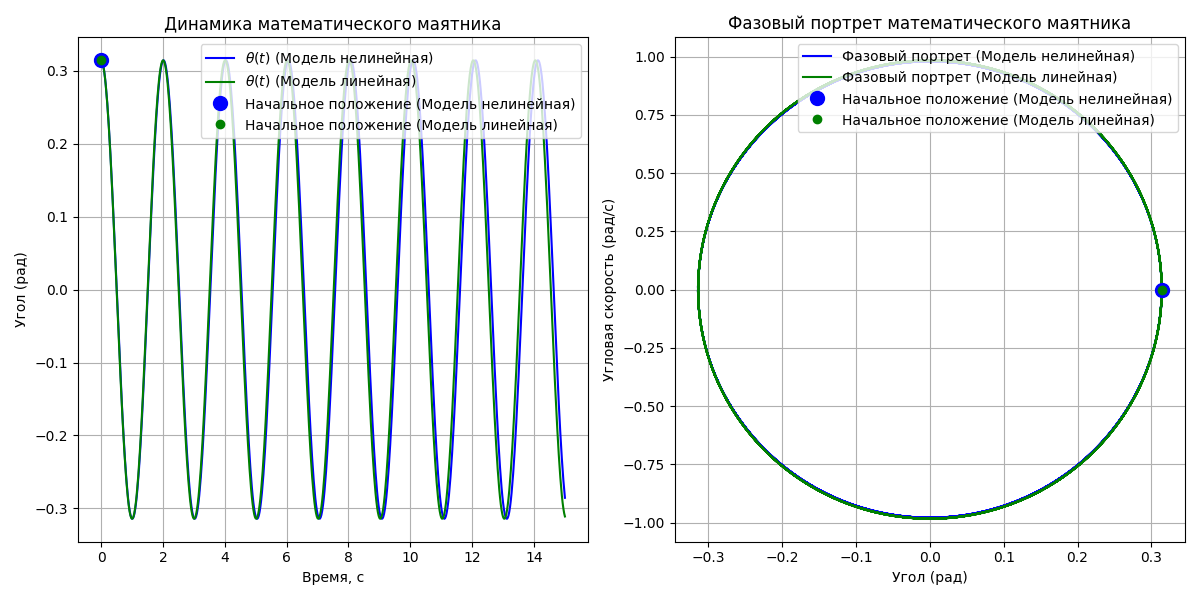
\includegraphics[width=1\textwidth]{imgs/pi10.png}  % Вставка изображения
	\caption{$\theta(0) = \pi / 10$.}  % Подпись к изображению
	\label{fig:pi10}  % Метка для ссылки
\end{figure}
\begin{figure}[h]  % Окружение для картинки
	\centering
	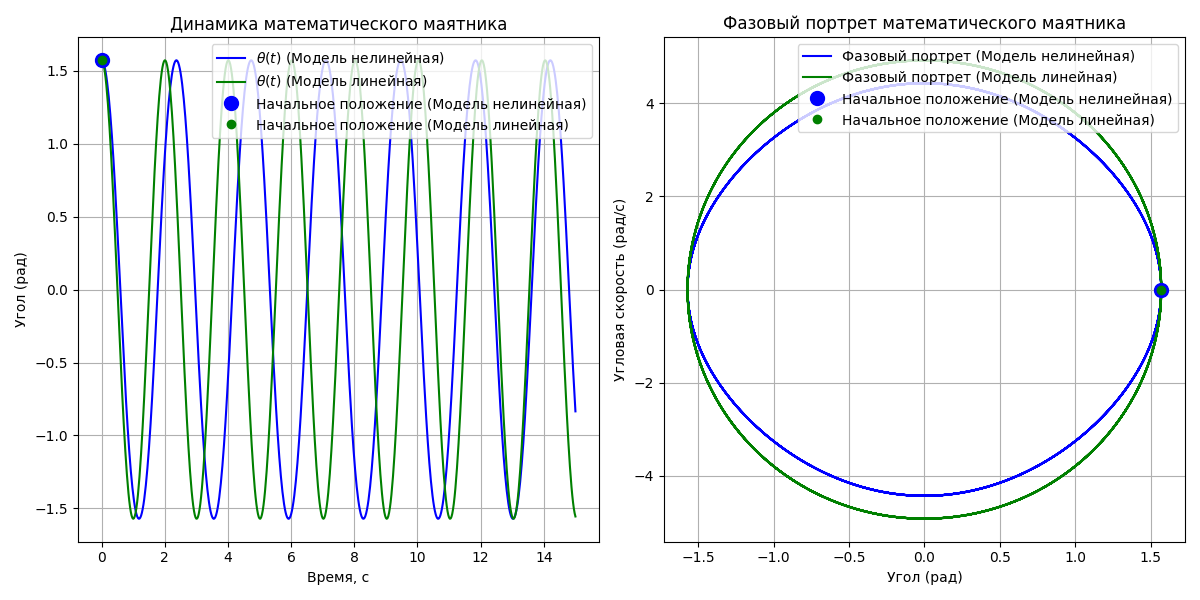
\includegraphics[width=1\textwidth]{imgs/pi2.png}  % Вставка изображения
	\caption{$\theta(0) = \pi / 2$.}  % Подпись к изображению
	\label{fig:pi2}  % Метка для ссылки
\end{figure}

Как видно на графиках (рис. \ref{fig:pi10}, \ref{fig:pi2}), при небольшом угле наклона разница между моделями не большая. При увеличении угла разница возрастает, что влечёт погрешность линейной модели. На фазовом портрете нелинейная модель имеет более узкий эллипс, что означает меньшую скорость. 

Для дальнейших экспериментов будем использовать линейную модель при малых отклонениях.

\newpage
\subsection*{Модель с трением}
Рассмотрим влияние трения на линейную модель про начальных условиях: $\theta(0) = \pi /10, \ \dot{\theta} = 0$. Промежуток времени $[0,40]$, шаг - 0.04:
\begin{figure}[h]  % Окружение для картинки
	\centering
	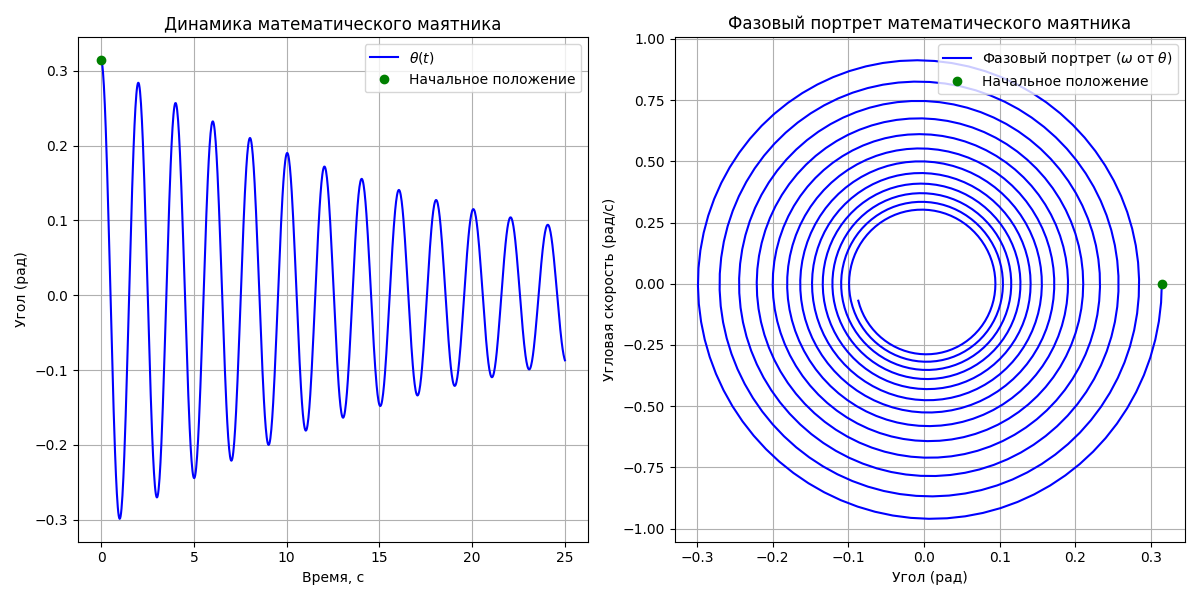
\includegraphics[width=1\textwidth]{imgs/lin_mu01.png}  % Вставка изображения
	\caption{$\mu = 0.1$.}  % Подпись к изображению
	\label{fig:mu_01}  % Метка для ссылки
\end{figure}

\begin{figure}[h]  % Окружение для картинки
	\centering
	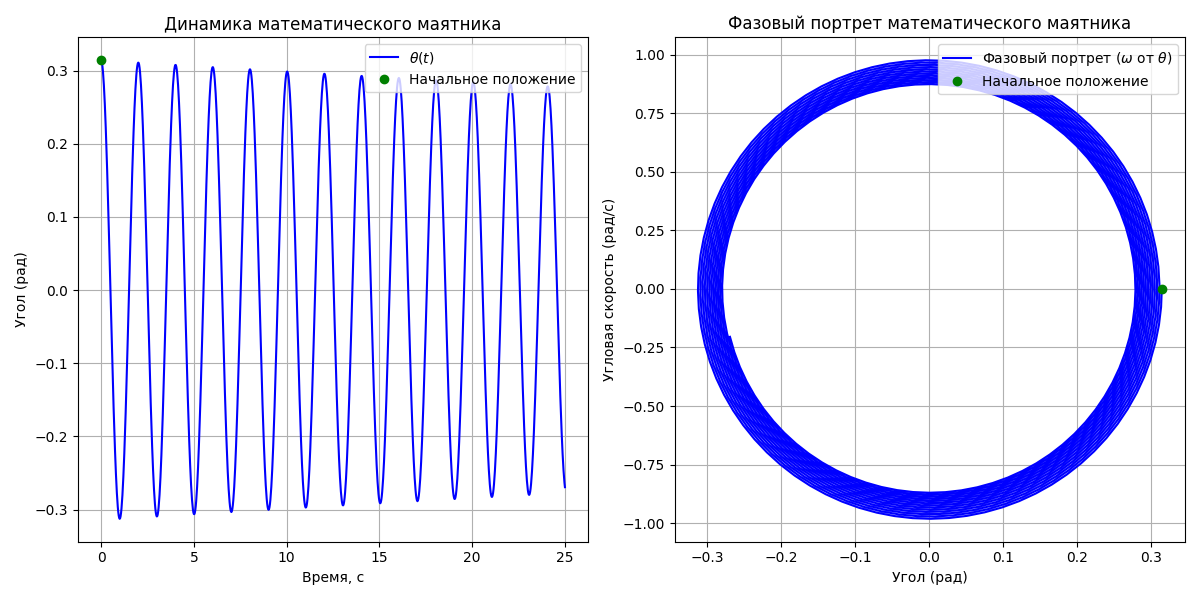
\includegraphics[width=1\textwidth]{imgs/lin_mu001.png}  % Вставка изображения
	\caption{$\mu = 0.01$.}  % Подпись к изображению
	\label{fig:mu_001}  % Метка для ссылки
\end{figure}

Результаты показывают (Рис. \ref{fig:mu_01}, \ref{fig:mu_001}). что под действием силы трения колебания становятся затухающими. Кривая на фозовой плоскости стремится к нулю. Чем больше коэффициент трения ($\mu$), тем быстрее затухают колебания.

\subsection*{Модель с вынужденными колебаниями}
Рассмотрим влияние внешней силы на линейную модель при начальных условиях: $\theta(0) = \pi /2, \ \dot{\theta} = 0$. Промежуток времени $[0,25]$, шаг - 0.025:
\begin{figure}[h]  % Окружение для картинки
	\centering
	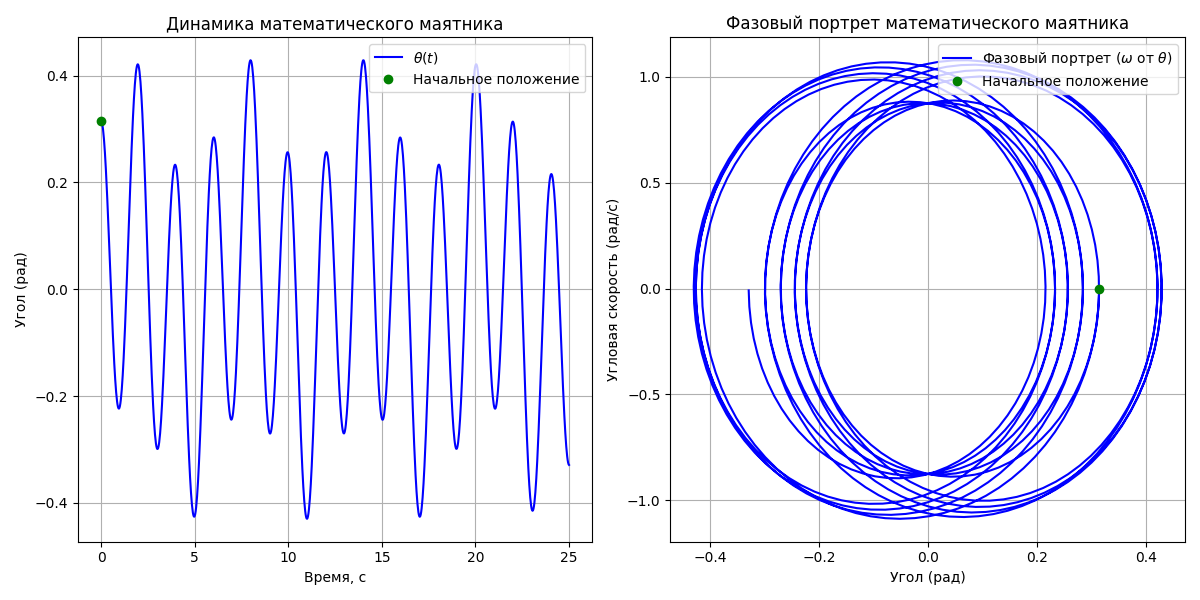
\includegraphics[width=1\textwidth]{imgs/f1w1.png}  % Вставка изображения
	\caption{$F_e = 1, \omega_f = 1$.}  % Подпись к изображению
	\label{fig:f1_w1}  % Метка для ссылки
\end{figure}

При воздействии внешних сил, происходит смещение значений угла наклона маятника, что отражается на фазовой плоскости (Рис. \ref{fig:f1_w1}).

\begin{figure}[h]  % Окружение для картинки
	\centering
	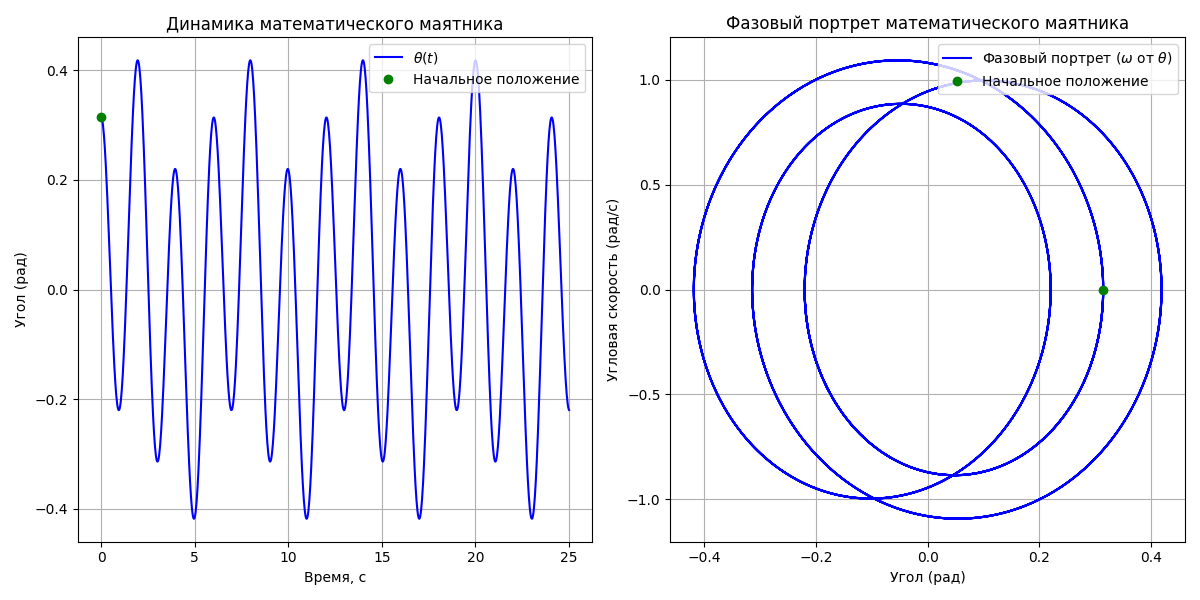
\includegraphics[width=1\textwidth]{imgs/f1ww3.png}  % Вставка изображения
	\caption{$F_e = 1, \omega_f = \omega/3$.}  % Подпись к изображению
	\label{fig:f1_ww3}  % Метка для ссылки
\end{figure}

При воздействии внешних сил с частотой, равной целой доли от собственной частоты маятника, на графике углов и фазовой плоскости видно (Рис. \ref{fig:f1_ww3}) периодичность колебаний.

\begin{figure}[h]  % Окружение для картинки
	\centering
	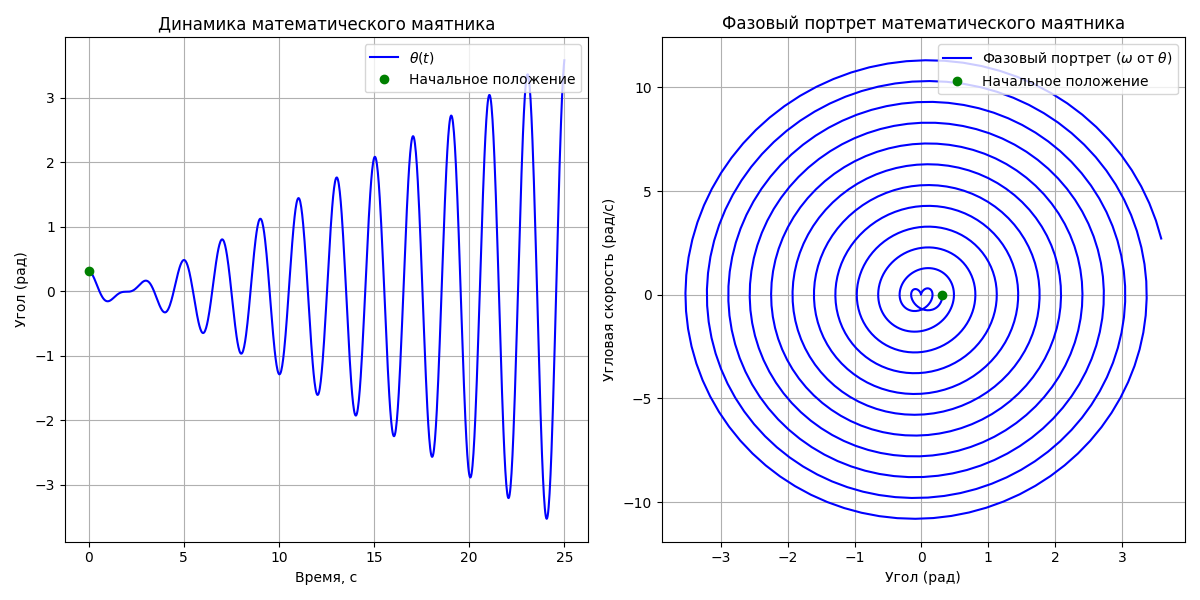
\includegraphics[width=1\textwidth]{imgs/f1ww.png}  % Вставка изображения
	\caption{$F_e = 1, \omega_f = \omega$.}  % Подпись к изображению
	\label{fig:f1_ww}  % Метка для ссылки
\end{figure}

В случае совпадения собственной частоты и частоты воздействия внешних сил, происходит эффект резонанса - аплитуда колебаний маятника неограниченной растёт (Рис. \ref{fig:f1_ww}).
\newpage
\subsection*{Модель с трением и вынужденными колебаниями}
Рассмотрим модель с обеими силами при начальных условиях: $\theta(0) = \pi /10, \ \dot{\theta} = 0$. Промежуток времени $[0,100]$, шаг - 0.1:
\begin{figure}[h]  % Окружение для картинки
	\centering
	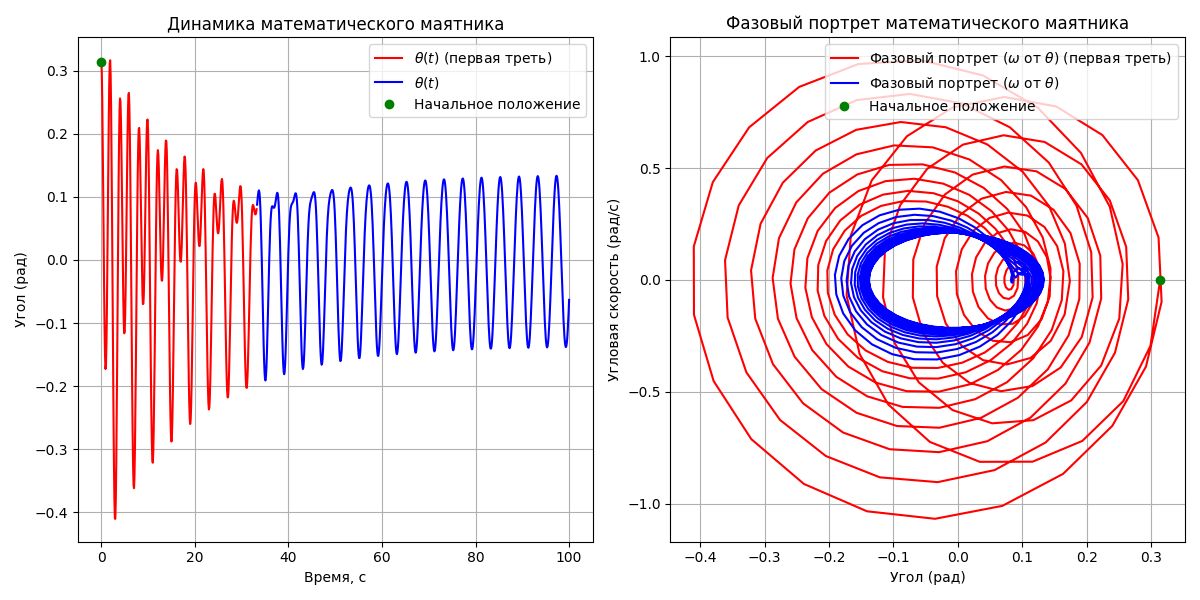
\includegraphics[width=1\textwidth]{imgs/f1w05mu01.png}  % Вставка изображения
	\caption{$F_e = 1, \omega_f = 0.5, \mu = 0.1$.}  % Подпись к изображению
	\label{fig:f1_w05_mu01}  % Метка для ссылки
\end{figure}

Изначальные хаотические колебания сглаживаются (Рис. \ref{fig:f1_w05_mu01}). Постепенно происходит смена частоты и амплитуды. 

\begin{figure}[h]  % Окружение для картинки
	\centering
	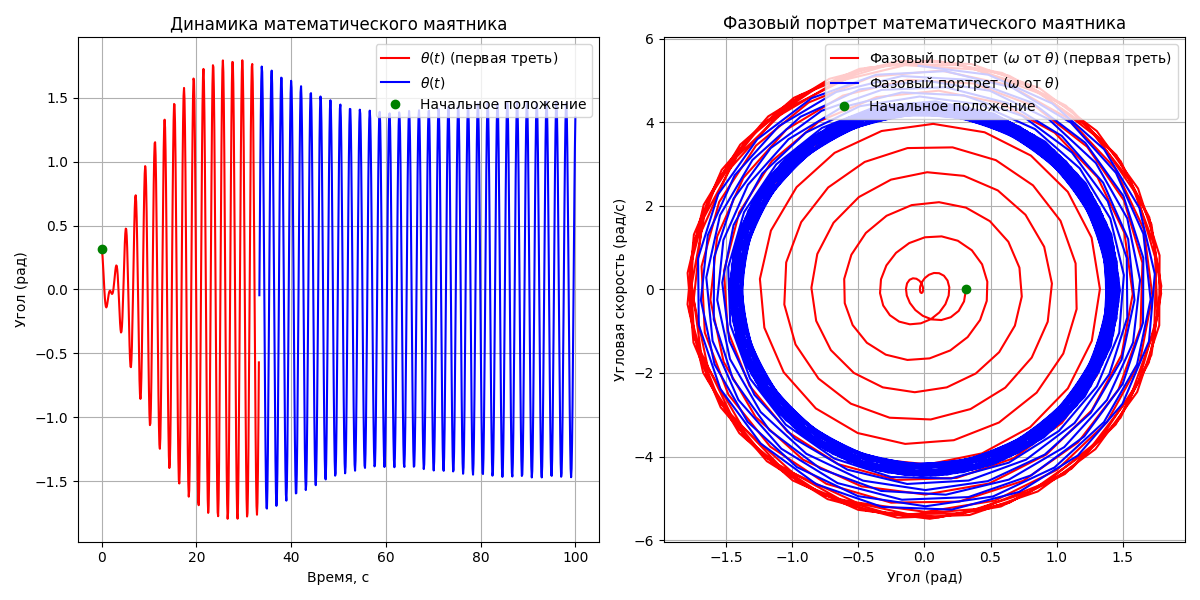
\includegraphics[width=1\textwidth]{imgs/f1ww-01mu01.png}  % Вставка изображения
	\caption{$F_e = 1, \omega_f = \omega - 0.1, \mu = 0.1$.}  % Подпись к изображению
	\label{fig:f1_w_mu01}  % Метка для ссылки
\end{figure}

При приближении к собственной частоте период и амплитуда устанавливаемых колебаний увеличиваются(Рис. \ref{fig:f1_w_mu01}).

\begin{figure}[h]  % Окружение для картинки
	\centering
	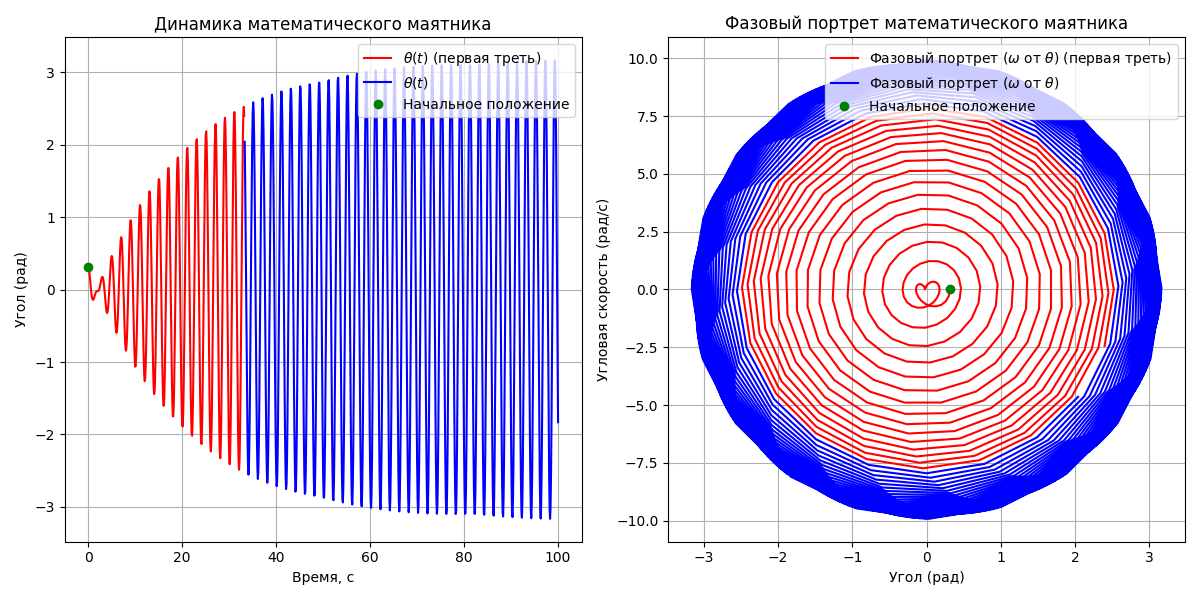
\includegraphics[width=1\textwidth]{imgs/tired.png}  % Вставка изображения
	\caption{$F_e = 1, \omega_f = \omega , \mu = 0.1$.}  % Подпись к изображению
	\label{fig:f1}  % Метка для ссылки
\end{figure}

В условиях резонанса достигается наибольшая амплитуда колебаний. В отличие от модели без учета трения, в данном случае амплитуда не будет расти бесконечно. Однако наличие силы трения не означает, что резонансная частота совпадает с собственной частотой системы.
\newpage

\subsection*{Резонанс}
Для исследования резонанса рассмотрим резонансные кривые. Т.к. этот эффект связан с частотой, то будем выбирать несколько значений частоты, вынуждающих калебания около неё. Для каждой из таких частот получим решение численным методом и найдём из последней четверти максимальное по модулю. Таким образом, мы получим зависимость $A=\theta(\omega_f)$. Для оценки точности сравним полученное значение с известной аналитической формулой\cite{feinman} (примем массу за 1 кг):
\begin{equation}
	\theta(\omega_f) = \frac{F_e}{m \sqrt{(2\omega_f \omega \zeta)^2 + (\omega ^ 2 - \omega_f^2)^2}}, \ \zeta = \frac{\mu}{2m\omega}.
\end{equation}

По горизонтальной оси будет откладывать $\omega_f / \omega$. В этом случае, резонансная частота будет при значении 1. Построим кривые для различных занчений $mu$ на отрезках $[0.5\omega, 2\omega]$ и $[0.9\omega, 1.1\omega]$, создав равномерную сетку из 60 точек.

\begin{figure}[h]  % Окружение для картинки
	\centering
	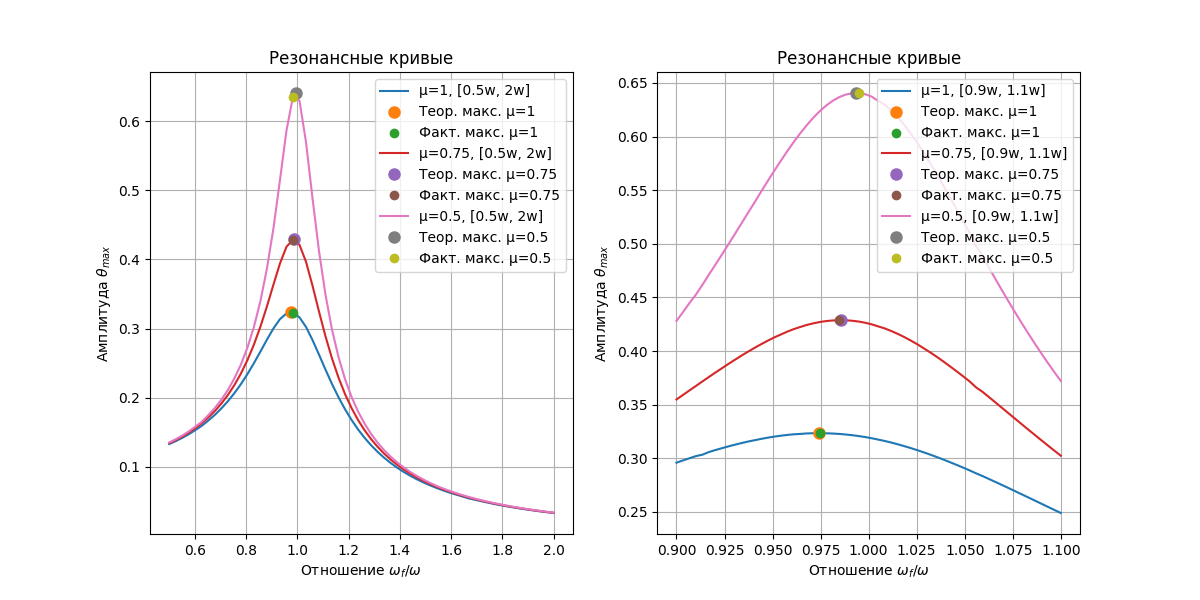
\includegraphics[width=1\textwidth]{imgs/res.png}  % Вставка изображения
	\caption{Кривая амплитуд.}  % Подпись к изображению
	\label{fig:res}  % Метка для ссылки
\end{figure}

Как можно видеть (Рис. \ref{fig:res}). Для разных коэффициентов трения резонансная частота достигается в разных местах. Отметим, что при уменьшении трения, амплитуда становится больше, и резонансная частота приближается к собственной. 


